\documentclass[../main.tex]{subfiles}
\begin{document}
	
	\section*{\underline{Section name:} Area of unknown shapes using known shapes}
	Calculate the area of the given figures.
	
	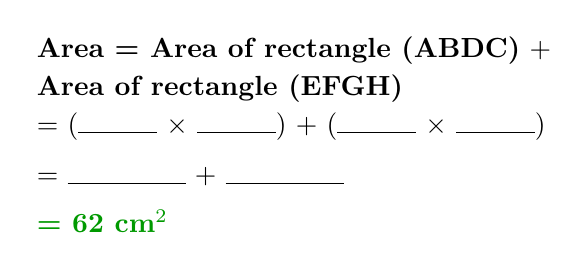
\begin{tikzpicture}[scale=0.8]
		\tkzDefPoint(0,5){A}
		\tkzDefPoint(3,5){B}
		\tkzDefPoint(3,3.5){E}
		\tkzDefPoint(6,3.5){F}
		\tkzDefPoint(6,1.8){G}
		\tkzDefPoint(0,0){D}
		\tkzDefPoint(3,0){C}
		\tkzDefPoint(3,1.8){H}
		
		\tkzDrawPolygon(A,B,E,F,G,H,C,D)
		
		\tkzLabelPoints[left](A,D)
		\tkzLabelPoints[above](B)
		\tkzLabelPoints[right](F,G,C)
		\tkzLabelPoints[below right](H)
		\tkzLabelPoints[above right](E)
		
		\tkzLabelSegment[auto](A,B){5 cm}
		\tkzLabelSegment[auto](E,F){6 cm}
		\tkzLabelSegment[left](A,D){10 cm}
		\tkzLabelSegment[auto](F,G){2 cm}
		
		\node[right] at (10,4) {\textbf{Area = Area of rectangle (ABDC)} +};
		\node[right] at (10,3.4) {\textbf{Area of rectangle (EFGH)}};
		\node[right] at (10,2.8) {= (\rule{1cm}{0.4pt} $\times$ \rule{1cm}{0.4pt}) + (\rule{1cm}{0.4pt} $\times$ \rule{1cm}{0.4pt})};
		\node[right] at (10,2) {= \rule{1.5cm}{0.4pt} + \rule{1.5cm}{0.4pt}};
		\node[right, text=green!60!black] at (10,1.3) {\textbf{= 62 cm$^2$}};
	\end{tikzpicture}\\
    [0.5cm]

    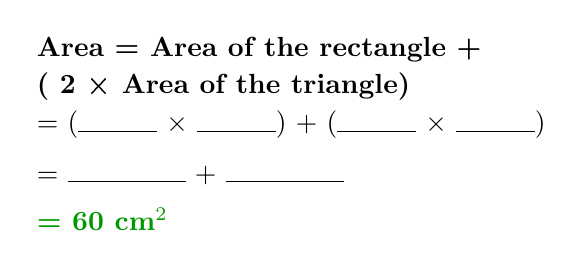
\begin{tikzpicture}[scale=0.8]
		\tkzDefPoint(3,6){L}
		\tkzDefPoint(6,6){M}
		\tkzDefPoint(8,3){N}
		\tkzDefPoint(6,0){O}
		\tkzDefPoint(3,0){P}
		\tkzDefPoint(1,3){Q}
		
		\tkzDrawPolygon(L,M,N,O,P,Q)
		
		\tkzLabelPoints[left](Q)
		\tkzLabelPoints[above](L,M)
		\tkzLabelPoints[right](N)
		\tkzLabelPoints[below](O,P)
		
		
		\tkzLabelSegment[above](L,M){2 cm}
		\tkzLabelSegment[right](M,N){4 cm}
		\tkzLabelSegment[right](N,O){4 cm}
		\tkzLabelSegment[below](P,O){2 cm}
		\tkzLabelSegment[left](Q,P){4 cm}
		\tkzLabelSegment[left](L,Q){4 cm}
		
		\node[right] at (12,4) {\textbf{Area = Area of the rectangle +}};
		\node[right] at (12,3.4) {\textbf{( 2 × Area of the triangle)}};
		\node[right] at (12,2.8) {= (\rule{1cm}{0.4pt} $\times$ \rule{1cm}{0.4pt}) + (\rule{1cm}{0.4pt} $\times$ \rule{1cm}{0.4pt})};
		\node[right] at (12,2) {= \rule{1.5cm}{0.4pt} + \rule{1.5cm}{0.4pt}};
		\node[right, text=green!60!black] at (12,1.3) {\textbf{= 60 cm$^2$}};
	\end{tikzpicture}\\
	
	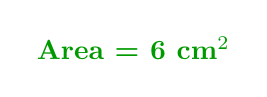
\begin{tikzpicture}[scale=0.8]
		\tkzDefPoint(0,5){A}
		\tkzDefPoint(2.5,5){B}
		\tkzDefPoint(2.5,2.5){C}
		\tkzDefPoint(7,2.5){D}
		\tkzDefPoint(7,0){E}
		\tkzDefPoint(0,0){G}
		\tkzDefPoint(3,0){F}
		
		\tkzDrawPolygon(A,B,C,D,E,F,G)
		
		\tkzLabelPoints[above](A,B,D)
		\tkzLabelPoints[above right](C)
		\tkzLabelPoints[below](E,F,G)
		
		\tkzLabelSegment[above](A,B){1 cm}
		\tkzLabelSegment[right](B,C){1 cm}
		\tkzLabelSegment[above](C,D){4 cm}
		\tkzLabelSegment[right](D,E){1 cm}
		\tkzLabelSegment[left](A,G){2 cm}
		
		\node[right, text=green!60!black] at (12,2) {\textbf{Area = 6 cm$^2$}};
	\end{tikzpicture}\\

    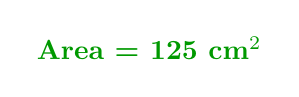
\begin{tikzpicture}[scale=0.8]
		\tkzDefPoint(0.5,4.5){M}
		\tkzDefPoint(2.5,6.5){N}
		\tkzDefPoint(4.5,4.5){O}
		\tkzDefPoint(6.5,6.5){P}
		\tkzDefPoint(8.5,4.5){Q}
		\tkzDefPoint(6.5,2.5){R}
		\tkzDefPoint(8.5,0.5){S}
		\tkzDefPoint(6.5,-1.5){T}
		\tkzDefPoint(4.5,0.5){U}
		\tkzDefPoint(2.5,-1.5){V}
		\tkzDefPoint(0.5,0.5){W}
		\tkzDefPoint(2.5,2.5){X}
		
		\tkzDrawPolygon(M,N,O,P,Q,R,S,T,U,V,W,X)
		
		\tkzLabelPoints[above](N,O,P,Q)
		\tkzLabelPoints[below](S,T,U,V)
		\tkzLabelPoints[right](R)
		\tkzLabelPoints[left](X,M,W)
		
		
		\tkzLabelSegment[left](M,N){5 cm}
        \tkzLabelSegment[right](N,O){5 cm}
        \tkzLabelSegment[right](P,Q){5 cm}
        \tkzLabelSegment[right](Q,R){5 cm}
        \tkzLabelSegment[right](S,T){5 cm}
        \tkzLabelSegment[below left](T,U){5 cm}
        \tkzLabelSegment[left](V,W){5 cm}
        \tkzLabelSegment[left](W,X){5 cm}
		
		
		\node[right, text=green!60!black] at (13,2) {\textbf{Area = 125 cm$^2$}};
	\end{tikzpicture}
	
	
\end{document}